\section{KNP tool}
KNP tool is a system which can perform parsing, case and anaphora analysis in Japanese texts.[4] It is provided by Kurohashi-Kawahara Laboratory of Kyoto University. It can use the parsing result of JUMAN system as the input and get dependency relationship, anaphora relationships, etc. It bases on a probability model which is automatically generated from the Web. In our research, We use KNP tool to extract the dependency case relationships between nouns and verbs. It lasts very long to analysis a long text, we need to divide the documents into short ones, or even sentences for a correct result. All of these have been done before our experiment. \\
After inputting a Japanese sentence, we can get a verb and the nouns that according to it. Verb, and nouns according to it, is the basis element of our research. We have a name of Event for it, we will have a detailed introduction in later Chapter. Here is a simple example of KNP result.\\
\begin{figure}[!h]
\centering
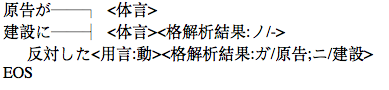
\includegraphics[width=250pt]{./pictures/0202.png}
\caption{a result of KNP tool}
\end{figure}
In our example, the original sentence is \begin{CJK}{UTF8}{ipxm}`原告が建設に反対した.'\end{CJK}, We can find that, in this sentence, the verb is \begin{CJK}{UTF8}{ipxm}`反対する'\end{CJK}, nouns are \begin{CJK}{UTF8}{ipxm}`原告'\end{CJK} and \begin{CJK}{UTF8}{ipxm}`建設'\end{CJK}, especially, \begin{CJK}{UTF8}{ipxm}`原告'\end{CJK} is in \begin{CJK}{UTF8}{ipxm}`が case'\end{CJK}, and \begin{CJK}{UTF8}{ipxm}`建設'\end{CJK} is in \begin{CJK}{UTF8}{ipxm}`に case'\end{CJK}. There are over 20 kinds of cases that can be extracted by KNP tool, in our research, we use some important ones, they are \begin{CJK}{UTF8}{ipxm}`ガ', `ヲ', `ニ', `ト', `デ', `カラ', `ヨリ', `マデ', `ヘ' and `時間'\end{CJK}. Because KNP comes from a big data from Web and uses a probability model, the correctness can be ensured. But KNP tool does nothing with passive sentences, We have to hand them by ourselves, for example, \\
\begin{CJK}{UTF8}{ipxm}  
`原告は被告を訴えた.'
\end{CJK}\\
\begin{CJK}{UTF8}{ipxm}
\CJKtilde  
`被告が原告に訴えられた.'
\end{CJK}
have the same meaning, but the cases of the nouns are totally different. We will have a transfer for passive sentences: 
\begin{enumerate}
\item \begin{CJK}{UTF8}{ipxm}`が case' to `よ case'\end{CJK}
\item \begin{CJK}{UTF8}{ipxm}`に case' to `が case'\end{CJK}
\item \begin{CJK}{UTF8}{ipxm}`による case' to `が case'\end{CJK}
\end{enumerate}
Although KNP is a very powerful tool, the result of KNP tool contains kinds of information. It is very hard for everyone to understand the result of KNP, and here I give an example to show how to read the output of KNP tool.\\ \\
\newpage
\textbf{Example of KNP}\\ \\
Input:\begin{CJK}{UTF8}{ipxm}麻生太郎はコーヒーを買って飲んだ。\end{CJK}\\
Option: -simple -anaphora\\
Output:\\
\begin{figure}[!h]
\centering
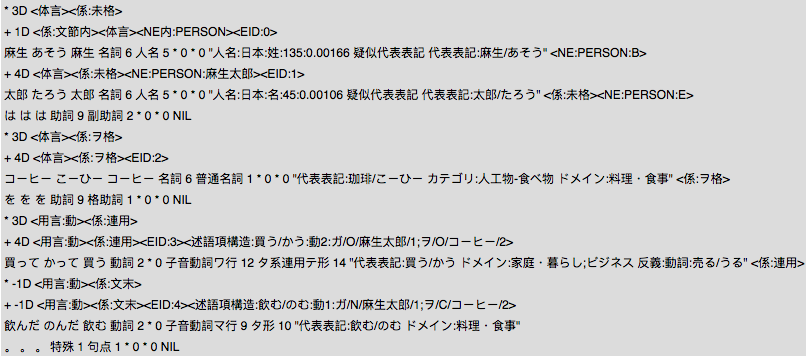
\includegraphics[width=350pt]{./pictures/0202-1.png}
\caption{example of KNP output}
\end{figure}
\\
Line starts with `$*$':
\begin{enumerate}
\item Information on clauses
\item In the case of the example in the example, the line beginning with "* 3D" at the head is ``Aso Taro'' (clause number = 0), the line beginning with ``* -1 D'' corresponds to``drunk'' (clause number = 3) 
\item The first digit represents the clause number (since the sentence at the end of the sentence does not have an affiliation, it is always output as ``-1'')
\item The following alphabet represents the type of dependency, and it is output as D for normal dependency relations, P for parallel etc.
\end{enumerate}
Line starts with `$+$'
\begin{enumerate}
\item Information on basic phrases
\item In KNP, basically it deals with dependency in the unit called "basic phrase consisting of one independent word and its adjunct
\item In terms of clause units ``Aso Tar'' becomes one clause, but when considered in basic phrase units, ``Aso'' and ``Taro'' are the two basic phrases
\item Forms such as dependency are the same as those starting with *
\end{enumerate}
After this transformation, almost all passive sentence can be correctly handled. From the detailed result of KNP, we can know whether a sentence is an active one or a passive one. Therefore, we can apply this transformation to convert our results.\\
KNP result will be our original data for our experiment.